\documentclass[12pt,a4paper]{report}
\usepackage[margin=25mm,headheight=15pt]{geometry}
\usepackage{graphicx,booktabs,amsmath,amssymb,longtable,array,tabularx,multirow}
\usepackage{caption,subcaption,float,xcolor,enumitem,fancyhdr,microtype,setspace}
\usepackage[hidelinks]{hyperref}
\usepackage{url}
\graphicspath{{report_assets/figures/}{report_assets/screenshots/}}
\definecolor{ink}{HTML}{111111}
\definecolor{rulegray}{HTML}{BFC5CC}
\hypersetup{pdftitle={Beyond Ranking Optimization Techniques Mini Project Report},pdfauthor={Bianca Sawant, Anushree Upasham, Ankita Sagar, Sofia Abidi}}
\captionsetup{font=small,labelfont=bf,justification=centering}
\setstretch{1.16}
\setlength{\parindent}{0pt}
\setlength{\parskip}{5pt}
\setcounter{secnumdepth}{3}
\setcounter{tocdepth}{2}
\renewcommand{\familydefault}{\sfdefault}
\makeatletter
\renewcommand{\@makechapterhead}[1]{\vspace*{8pt}{\parindent\z@\raggedright\normalfont\Huge\bfseries\color{ink}\thechapter\quad #1\par\nobreak\vskip 24pt}}
\renewcommand{\@makeschapterhead}[1]{\vspace*{8pt}{\parindent\z@\raggedright\normalfont\Huge\bfseries\color{ink}#1\par\nobreak\vskip 24pt}}
\makeatother
\pagestyle{fancy}\fancyhf{}\fancyhead[L]{\small VJTI Mumbai | Optimization Techniques}\fancyhead[R]{\small Beyond Ranking}\fancyfoot[L]{\small Bianca Sawant et al.}\fancyfoot[R]{\small Page \thepage}\renewcommand{\headrulewidth}{0.4pt}
\newcommand{\evidencewarning}{\begin{center}\small\textbf{Evidence boundary:} Synthetic and public-calibrated outputs are modeled decision-support evidence, not observed or causal VJTI improvements.\end{center}}
\newcommand{\artifact}[1]{\texttt{\detokenize{#1}}}

\begin{document}
\begin{titlepage}
\thispagestyle{empty}
\begin{center}
{\large\bfseries VEERMATA JIJABAI TECHNOLOGICAL INSTITUTE\par}
{\large VJTI, Mumbai\par}
\vspace{1.3cm}
{\Large\bfseries OPTIMIZATION TECHNIQUES\par}
{\Large\bfseries MINI PROJECT REPORT\par}
\vspace{1.7cm}
{\Huge\bfseries BEYOND RANKING\par}
\vspace{0.35cm}
{\Large\itshape A Data-Driven Multi-Objective Framework for VJTI CE \& IT Department Productivity\par}
\vspace{1.5cm}
{\large Department of Computer Engineering \& Information Technology\par}
\vspace{1.1cm}
{\large\bfseries Submitted by\par}\vspace{0.35cm}
\begin{tabular}{ll}
Bianca Sawant & 241071067\\
Anushree Upasham & 241071077\\
Ankita Sagar & 241071063\\
Sofia Abidi & 241071075
\end{tabular}
\vfill
{\large Academic Year 2026--2027\par}
\end{center}
\end{titlepage}

\pagenumbering{roman}
\tableofcontents
\clearpage
\listoffigures
\clearpage
\listoftables
\clearpage

\chapter*{Team Members and Individual Contributions}
\addcontentsline{toc}{chapter}{Team Members and Individual Contributions}
\begin{longtable}{p{0.21\textwidth}p{0.25\textwidth}p{0.46\textwidth}}
\toprule
\textbf{Member} & \textbf{Role} & \textbf{Documented responsibility}\\ \midrule
Ankita Sagar (241071063) & Algorithm Development \& Optimization & Development and refinement of multi-objective algorithms, including the hybrid RION method and implementations of NSGA-II, NSGA-III, MOPSO, and MOEA/D; constraint-aware search, debugging, and common-framework comparison.\\
Sofia Abidi (241071075) & ML Modeling \& System Integration & DEA benchmarking, KPI prediction models, linkage of prediction and resource allocation, comparative benchmarking support, model-output verification, and integration testing.\\
Anushree Upasham (241071077) & Research \& System Architecture & Literature foundation, KPI identification, four objective families, controllable variables, resource constraints, mathematical formulation, and conceptual architecture.\\
Bianca Sawant (241071067) & Strategic Analysis \& Experimental Design & Budget scenarios, evaluation metrics, robustness and sensitivity protocols, Pareto analysis, strategy interpretation, and validation methodology.\\ \bottomrule
\end{longtable}

The report treats these as team responsibilities supplied for this submission. It does not infer undocumented authorship from file history. Ankita's role centers on making distinct search methods comparable without changing the common feasibility semantics. Sofia's work connects descriptive efficiency analysis and predictive models to the evaluation contract while preserving validation gates. Anushree's contribution establishes what is optimized and why the decisions, objectives, and constraints are institutionally meaningful. Bianca's contribution defines how claims are tested, compared, and translated into planning alternatives rather than a single unqualified ``best'' allocation.

\chapter*{Abstract}
\addcontentsline{toc}{chapter}{Abstract}
Beyond Ranking is a reproducible multi-objective decision-support system for departmental resource allocation. The implemented system validates data and provenance, performs gated data-envelopment analysis (DEA), trains and audits KPI response models, repairs and evaluates mixed-variable allocations, executes six optimization algorithms through one canonical evaluator, compares algorithms under matched budgets, tests structural and stochastic robustness, and exposes saved and live results through FastAPI and Streamlit. The final synthetic benchmark contains 150 completed jobs from six algorithms and 25 seeds. MOPSO achieved the highest median hypervolume (0.0006862869) and lowest median IGD (0.0052269), while MOEA/D was statistically indistinguishable from MOPSO after Holm correction. These findings concern a frozen synthetic fixture whose innovation, student, and societal objectives are unsupported zeros. A separate public-calibrated VJTI scenario represents all four objective families but uses synthetic response functions; its 18 completed runs are not empirical validation. The current software passes 84 of 84 available backend tests with six optional native OpenMP tests skipped, and all 53 Streamlit/API tests. The system therefore demonstrates a complete optimization and explanation workflow while explicitly withholding causal or empirically validated policy claims.
\evidencewarning

\clearpage\pagenumbering{arabic}
\chapter{Introduction}
Higher-education departments must distribute limited money, faculty effort, research assistance, and infrastructure across competing responsibilities. Research output, innovation, student development, and societal contribution can all be desirable, but they draw on shared capacity and cannot be maximized independently. Rankings intensify this tension, yet improving a ranking indicator is not identical to improving educational value. The implemented project therefore reframes ``rank improvement'' as a constrained resource-allocation problem with explicit objectives, uncertainty, provenance, and evidence limits.

The original proposal introduced RION, a hybrid NSGA-II and particle-swarm approach. The repository now contains a broader research pipeline: schemas and manifests; a BCC/VRS DEA implementation; baseline, linear, and Random Forest response models; deterministic mixed-variable repair; six optimizers; matched-budget benchmarking; paired statistical tests; robustness analysis; reverse target-cost search; public-data packaging; independent audits; and a presentation-oriented dashboard. This report documents that implemented system rather than repeating the proposal.

The central design principle is evaluator reuse. Every algorithm submits a candidate allocation to the same problem object. That evaluator decodes and repairs decisions, predicts KPIs and intervals, computes four objective-family benefits, checks named constraints, and emits evidence metadata. Reporting and the dashboard consume saved evaluator outputs or call the backend; neither duplicates scientific logic.

\section{Scope and research questions}
The project asks: (i) how can a department formulate competing allocation goals without optimizing observed outcomes directly; (ii) how do six search strategies compare under equal candidate-evaluation budgets; (iii) how stable are selected strategies under budget, capacity, cost, and predictive uncertainty; and (iv) how can results be explained live without converting modeled associations into causal claims?

\chapter{Problem Statement and Objectives}
Let $x$ be a mixed vector of controllable decisions and $c$ the fixed scenario context. The system seeks feasible nondominated allocations rather than a single scalar optimum:
\begin{equation}
\min_{x\in\mathcal{X}}\;F(x;c)=\big[-B_R(x),-B_I(x),-B_S(x),-B_C(x)\big],
\end{equation}
where $B_R$, $B_I$, $B_S$, and $B_C$ are normalized modeled benefits for research, innovation, student development, and societal contribution. Cost is a hard constraint and reporting dimension, not a fifth objective.

The implemented objectives are to build an auditable data layer; prevent observed, derived, synthetic, and unsupported values from being conflated; provide a shared evaluator; compare six genuine algorithm adapters; quantify convergence, proximity, spread, feasibility, and runtime; test strategy robustness; support reverse target-cost exploration; and provide an understandable live interface with downloadable provenance.

The VJTI public-calibrated evaluator contains 12 decisions: seven funding allocations, three faculty-effort allocations, research-assistant count, and compute-capacity units. The legacy synthetic evaluator contains five decisions and supports research only. Predicted publications, citations, placements, patents, and outreach are outputs, never decision variables.

\chapter{Literature Review}
Multi-objective evolutionary optimization is appropriate when objectives conflict and the decision maker requires a set of trade-offs. NSGA-II uses elitist nondominated sorting and crowding distance \cite{deb2002nsga2}. NSGA-III extends this family with reference directions and niching for many-objective search \cite{deb2014nsga3}. MOEA/D decomposes the vector problem into neighboring scalar subproblems \cite{zhang2007moead}. Multi-objective particle swarm methods use leaders from a bounded nondominated archive \cite{coello2004mopso}. The project implements these ideas natively so all methods can use the repository's repair and constraint contract.

DEA estimates a relative efficiency frontier rather than a causal production function. The implementation uses an input-oriented variable-returns-to-scale model associated with the BCC formulation \cite{banker1984dea}; the earlier CCR work established the core linear-programming frontier approach \cite{charnes1978dea}. A score indicates radial efficiency relative to a selected cohort and variable set. It does not prove that resources can be removed in practice.

For repeated algorithm comparison, the project uses paired Wilcoxon signed-rank tests \cite{wilcoxon1945}, rank-biserial effects, and Holm correction \cite{holm1979}. This is superior to comparing only best runs. Still, statistical significance on a synthetic fixture is not evidence of institutional impact.

\chapter{System Architecture and Methodology}
\begin{figure}[H]\centering
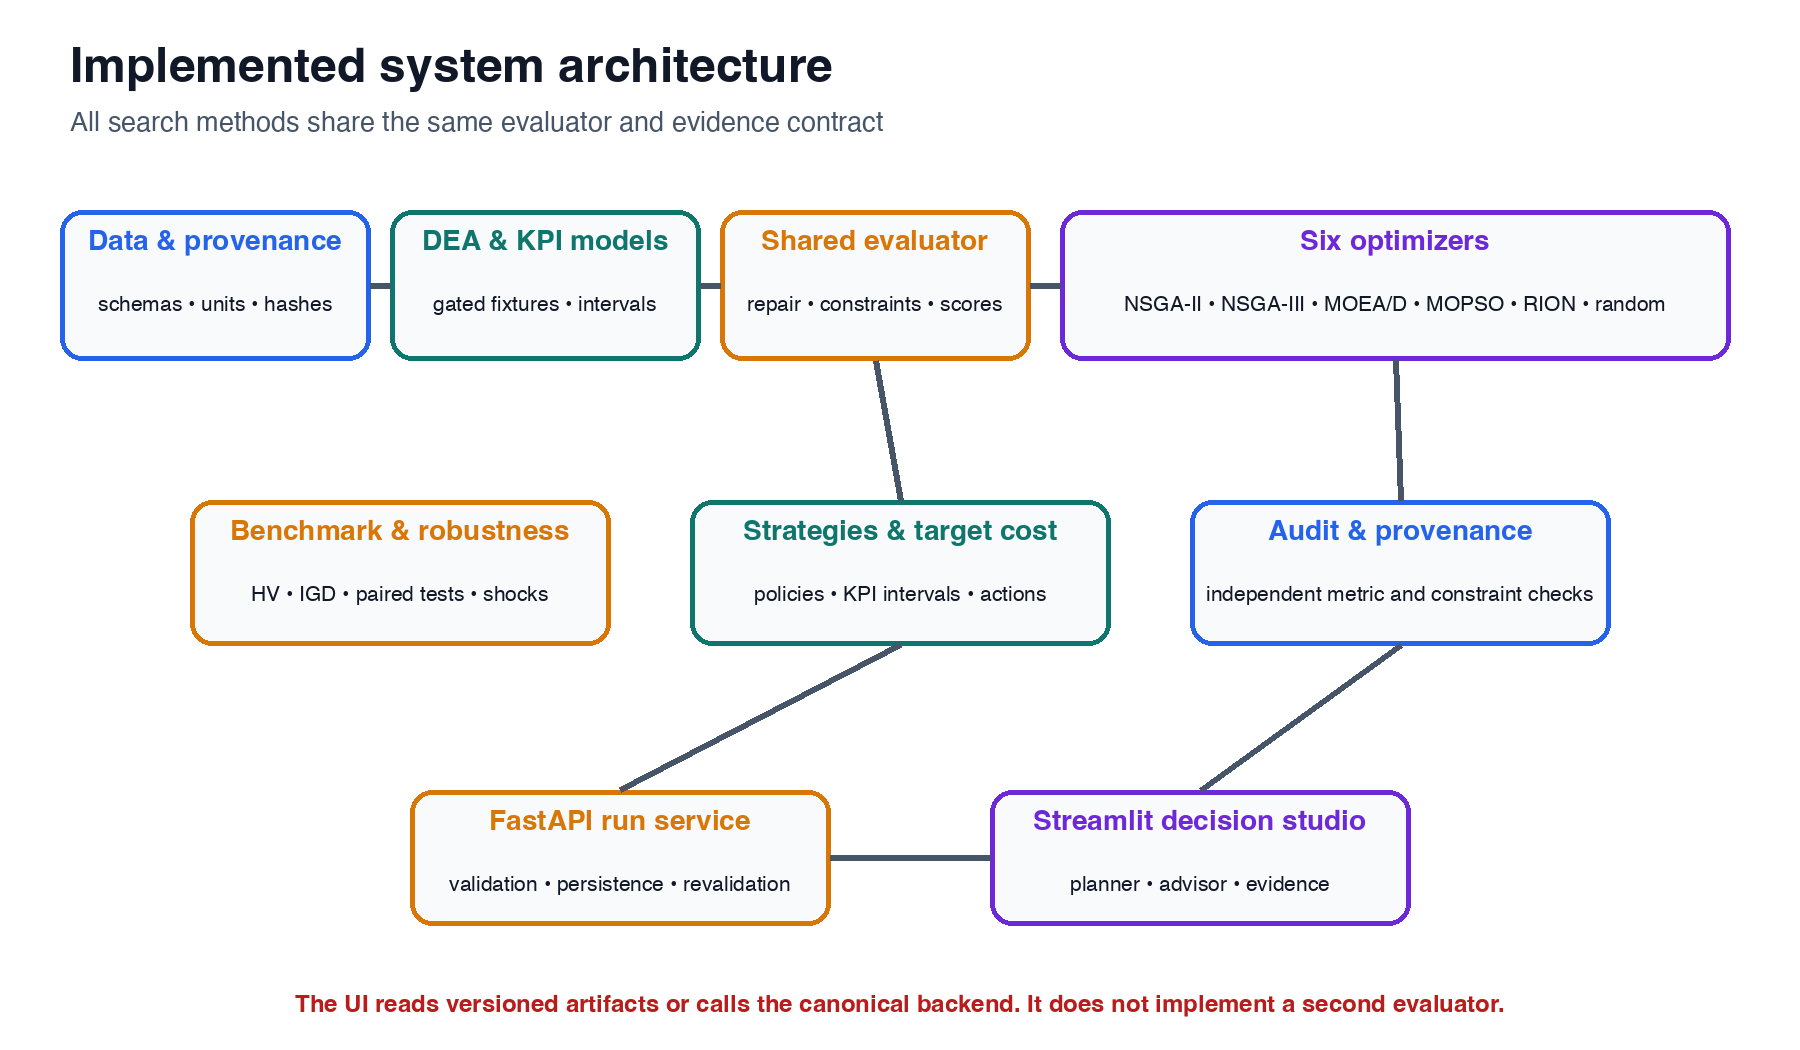
\includegraphics[width=\textwidth]{system_architecture.png}
\caption{Implemented Beyond Ranking architecture. The canonical evaluator is shared by all six algorithms and live dashboard runs.}
\end{figure}

The data workflow validates required fields, units, identifiers, numerical finiteness, bounds, allocation semantics, and source conflicts. Manifests store SHA-256 fingerprints. DEA and KPI modeling are evidence-gated. The evaluator applies deterministic repair before prediction and feasibility checks. Optimizers return populations and feasible nondominated archives in one schema. Benchmarking freezes metric normalization and evaluation budgets before runs. Strategy selection is post-optimization and records its rule. Audit modules independently recompute selected predictions, constraints, Pareto status, hypervolume, and IGD.

The public-data package retains seven immutable official snapshots and 12 reproducible searches. Institute-level values are never silently converted into department observations. Public values can calibrate baselines or targets, but response relationships remain synthetic unless department-period evidence supports validation.

\chapter{Dataset, DEA and KPI Predictive Modeling}
\section{Evidence lanes}
Three evidence lanes are maintained. The legacy synthetic fixture has 521 generated records and is used for method tests. The public-calibrated VJTI package combines official descriptive facts with a labeled synthetic scenario generator. The empirical lane contains observed or derived public values but currently has no longitudinal allocation-outcome panel. Consequently, it contains no empirically validated optimizer result.

\begin{table}[H]\centering\small
\caption{Evidence classes used by the implementation.}
\begin{tabularx}{\textwidth}{p{0.22\textwidth}X X}\toprule
Class & Meaning & Permitted claim\\\midrule
Observed public & Directly transcribed official value with source scope and period & Descriptive fact only\\
Derived public & Transparent arithmetic from public values & Descriptive derived fact\\
Synthetic scenario & Generated or calibrated response used for method testing & Modeled scenario behavior\\
Unsupported & Missing evidence or model support & Explicitly blocked conclusion\\\bottomrule
\end{tabularx}
\end{table}

\section{DEA}
For evaluated unit $o$, the input-oriented VRS envelopment model is
\begin{align}
\min_{\theta,\lambda}\quad &\theta\\
\text{s.t.}\quad &\sum_j\lambda_jx_{ij}\leq \theta x_{io},\quad\forall i,\\
&\sum_j\lambda_jy_{rj}\geq y_{ro},\quad\forall r,\\
&\sum_j\lambda_j=1,\quad\lambda_j\geq0.
\end{align}
The 521-unit legacy fixture solved all LPs and identified 57 strongly efficient units (10.94\%). A separate 30-unit calibrated synthetic fixture also solved completely. Public DEA is blocked because there are zero sufficiently complete comparable public DMUs against the configured minimum of 12.

\section{KPI response models}
Mean, linear, and Random Forest candidates are compared on disjoint train, validation, calibration, and later-period test splits. Median imputation and scaling reside inside fitted pipelines, preventing preprocessing leakage. Nine KPIs are modeled in the calibrated fixture. Selected test MAEs include 0.885 for Q1 publications, 0.0492 for normalized citation impact, 0.285 for patent applications, 2.829 for placements, and 4.554 for student research participants. These validate recovery of the synthetic generator, not VJTI intervention effects. Split-conformal intervals use eight calibration and eight test observations per KPI, so coverage estimates are imprecise and remain labeled synthetic.

\chapter{Mathematical Formulation and Constraints}
Each objective family combines supported KPI components after configured min--max normalization:
\begin{equation}
B_k(x)=\sum_{m\in\mathcal{M}_k}w_{km}\,z_{km}(\widehat{y}_m(x)),\qquad \sum_m w_{km}=1.
\end{equation}
Normalization values are stored in configuration and are not invented by the UI. The legacy benchmark maps internal scores from $[-1,0]$ to $[0,1]$ for metrics only; the evaluator itself does not silently clip normalized benefits.

Feasibility uses a uniform residual convention: $g_j(x)\leq0$ satisfies constraint $j$. Aggregate violation is
\begin{equation}
V(x)=\sum_j\frac{\max(0,g_j(x))}{s_j},
\end{equation}
where $s_j$ is a declared physical scale. Feasibility-first dominance prefers lower violation; among equally feasible candidates, ordinary Pareto dominance applies.

Constraints cover bounds, increments, integrality, total budget, faculty capacity, teaching/student/service floors, funding dependencies, and conservative KPI service thresholds. Repair clips and snaps values, enforces integer types, reduces faculty effort when capacity is exceeded, removes unsupported dependent counts, and reduces monetary variables in a declared priority order. Every repaired candidate is re-evaluated. Model-support flags remain separate from mathematical feasibility.

\begin{table}[H]\centering\small
\caption{Public-calibrated reference resource accounting.}
\begin{tabular}{lrr}\toprule Item & Value & Interpretation\\\midrule
Budget limit & INR 36.0 million & Hard scenario limit\\
Reference cost & INR 33.3 million & 92.5\% utilization\\
Budget headroom & INR 2.7 million & Remaining modeled capacity\\
Allocated faculty effort & 9.60 FTE & Across three activity categories\\
Decision variables & 12 & Mixed continuous, integer, and incremented\\\bottomrule
\end{tabular}
\end{table}

\chapter{Multi-Objective Optimization Algorithms}
\section{NSGA-II and NSGA-III}
NSGA-II uses tournament selection, simulated binary crossover, polynomial mutation, fast nondominated sorting, and crowding distance. NSGA-III uses the same variation framework but associates normalized candidates with deterministic Das--Dennis reference directions and fills underrepresented niches. Four objectives with three partitions yield 20 directions in the saved protocol.

\section{MOEA/D and MOPSO}
MOEA/D assigns one subproblem to each reference direction and uses a weighted Tchebycheff scalarization with the evolving ideal point. Parents come from neighboring weight vectors, and feasibility-first dominance precedes scalar replacement. MOPSO maintains positions, velocities, personal bests, and a bounded external archive. Leaders are selected by crowding distance; duplicate and dominated allocations are removed before pruning.

\section{RION and random search}
RION is the corrected hybrid inherited from the proposal. Its outer evolutionary loop uses NSGA-II selection, while an inner particle swarm mutates a selected decision coordinate with a row-aware objective and constraint penalty. Inner swarm evaluations are counted in the matched candidate budget. The serial backend is fully tested; the optional OpenMP library is absent in this workspace, so six native-only tests are skipped. Random search samples repaired candidates uniformly and provides a non-adaptive sanity baseline.

\begin{table}[H]\centering\small
\caption{Six algorithms under the common evaluator.}
\begin{tabularx}{\textwidth}{lX X}\toprule Method & Primary search mechanism & Diversity / comparison role\\\midrule
NSGA-II & Nondominated sorting and genetic variation & Crowding distance\\
NSGA-III & Reference-direction evolutionary search & Niching across directions\\
MOEA/D & Neighboring scalar decompositions & Weight-vector neighborhoods\\
MOPSO & Particle velocities and archive leaders & Crowding-pruned external archive\\
RION & NSGA-II with PSO-driven coordinate mutation & Proposal hybrid, corrected accounting\\
Random search & Uniform repaired sampling & Non-adaptive baseline\\\bottomrule
\end{tabularx}
\end{table}

\chapter{System Implementation and Dashboard}
FastAPI validates allowlisted scenario changes, launches an existing optimizer adapter, persists status and accounting, independently revalidates candidates, and returns recommendation facts. Streamlit provides Department Overview, Resource Planner, Improvement Advisor, Strategy Comparison, Experiment Lab, and Evidence \& Assumptions. The dashboard preserves exact technical tables inside expanders while showing rounded metrics and plain explanations in the main flow.

\IfFileExists{report_assets/screenshots/dashboard_overview.png}{\begin{figure}[H]\centering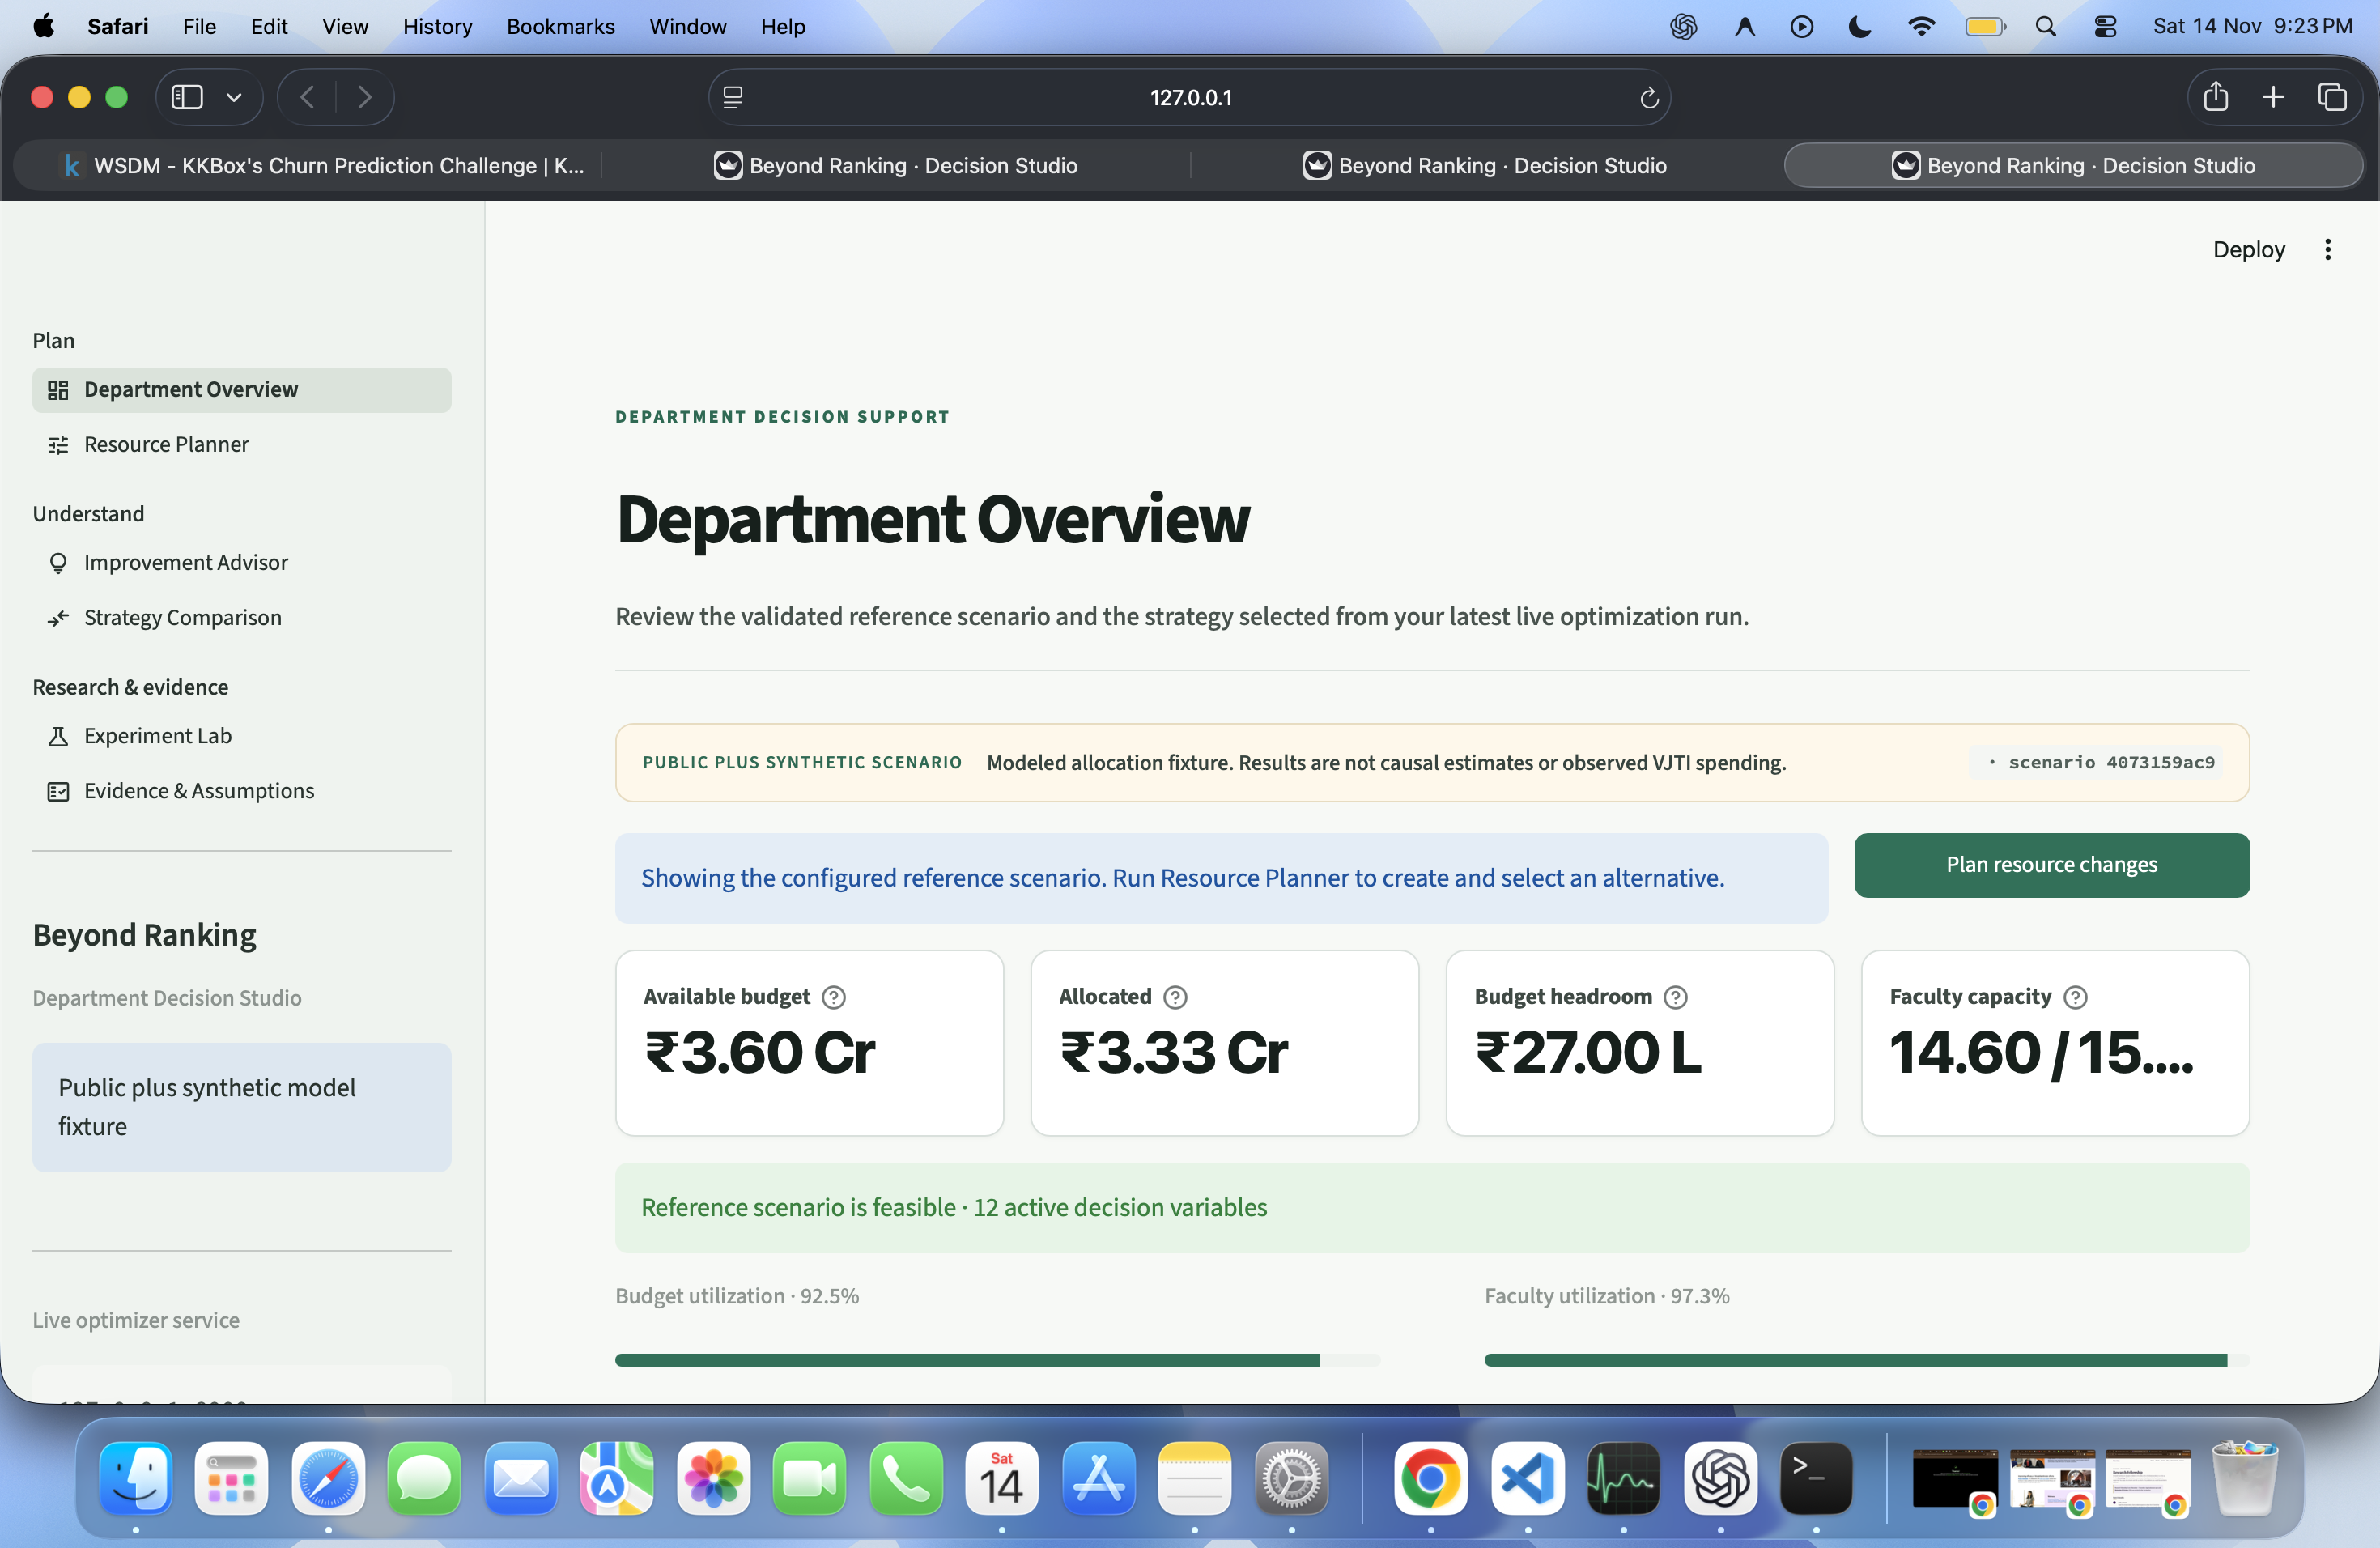
\includegraphics[width=\textwidth]{dashboard_overview.png}\caption{Authentic running Streamlit Department Overview showing the public-plus-synthetic evidence label, budget, headroom, feasibility, and utilization.}\end{figure}}{}

The Resource Planner exposes only backend-supported controls and validates units before execution. Improvement Advisor deterministically selects independently revalidated feasible candidates under declared balanced, research, innovation, student, and conservative profiles. It displays the largest meaningful allocation changes as action cards, including current and proposed values, units, change direction, constraints, trade-offs, and uncertainty. Duplicate profile selections and zero-change strategies are disclosed.

The optional Groq service is isolated after recommendation selection. It receives only an allowlisted structured fact packet. It cannot run an optimizer, select allocations, read arbitrary files, or calculate quantities. Provider output must satisfy local schemas and grounding checks; timeouts, malformed responses, unsupported causal language, or missing credentials trigger deterministic fallback wording. Credentials are never written to audit records.

\chapter{Experimental Setup}
The final synthetic benchmark freezes six algorithms, 25 non-tuning seeds, and 100 candidate evaluations per algorithm--seed job. Thus 150 jobs consume exactly 15,000 candidate evaluations with zero final-batch overshoot. Objective order, score bounds, and the hypervolume reference point $[1.1,1.1,1.1,1.1]$ are frozen in configuration. IGD uses a hashed pooled nondominated union because no true departmental Pareto front is known.

Metrics are hypervolume (higher is better), IGD (lower), nearest-neighbor spacing (lower, with zero for a one-point archive), feasible population rate, archive size, runtime, candidate evaluations, and unique evaluator calls. Paired two-sided Wilcoxon tests are performed only when at least ten matched successful seeds exist. Rank-biserial effects record direction and magnitude; Holm adjustment controls familywise multiplicity.

The separate public-calibrated comparison uses six algorithms, three seeds, and 16 candidate evaluations per run, producing 18 completed runs. It is a small scenario protocol, not the final algorithm ranking experiment.

\chapter{Results and Statistical Analysis}
\begin{figure}[H]\centering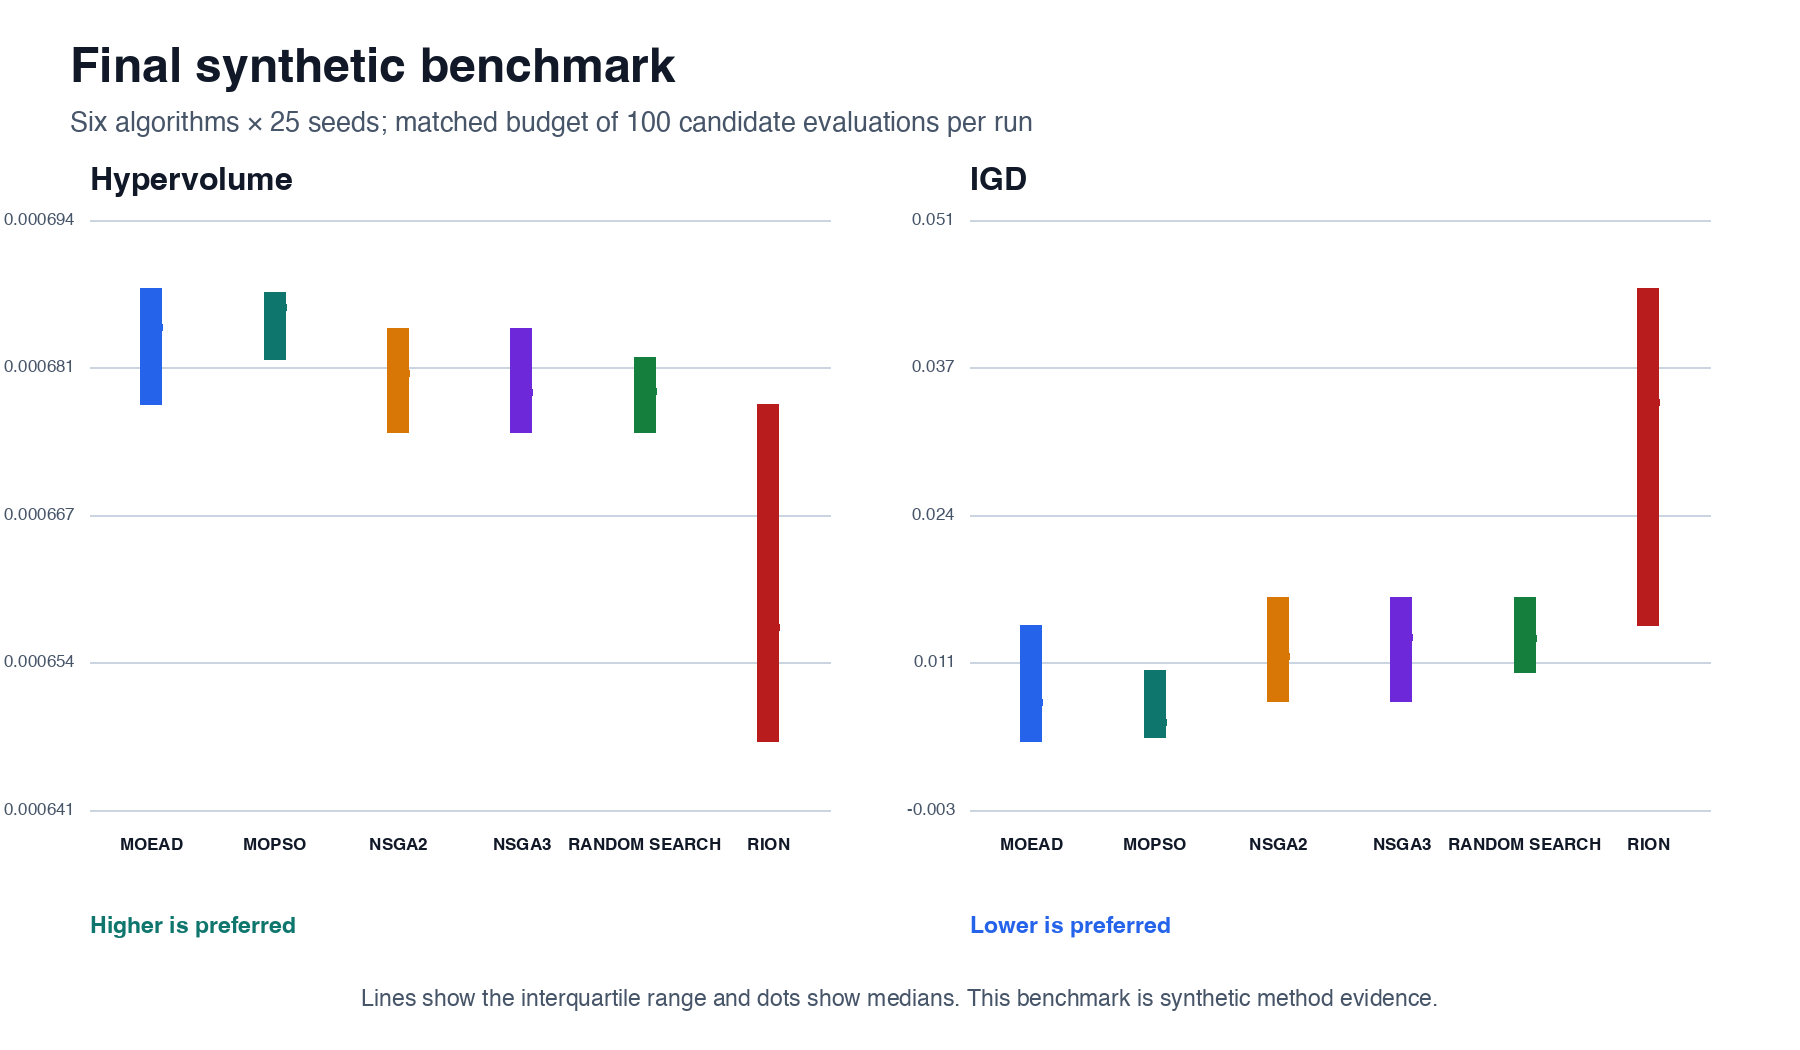
\includegraphics[width=\textwidth]{benchmark_comparison.png}\caption{Final synthetic benchmark hypervolume and IGD medians with interquartile ranges.}\end{figure}

MOPSO had median hypervolume 0.0006862869 and median IGD 0.0052269. MOEA/D followed with 0.0006844762 and 0.0070377. NSGA-II and NSGA-III medians were near 0.000680 and 0.000679, while RION had 0.000657 and IGD 0.034237. All six methods had median feasible-solution rate 1.0.

Holm-adjusted paired tests did not distinguish MOPSO from MOEA/D at 0.05. MOPSO was significantly better on hypervolume and IGD than NSGA-II, NSGA-III, random search, and RION. For example, MOPSO versus RION gave adjusted $p=0.000098$ with absolute rank-biserial effect 0.913846. MOEA/D versus RION gave adjusted $p=0.005384$ with effect 0.753846. The symmetry of hypervolume and IGD results arises because this fixture effectively varies only the supported research objective.

\begin{figure}[H]\centering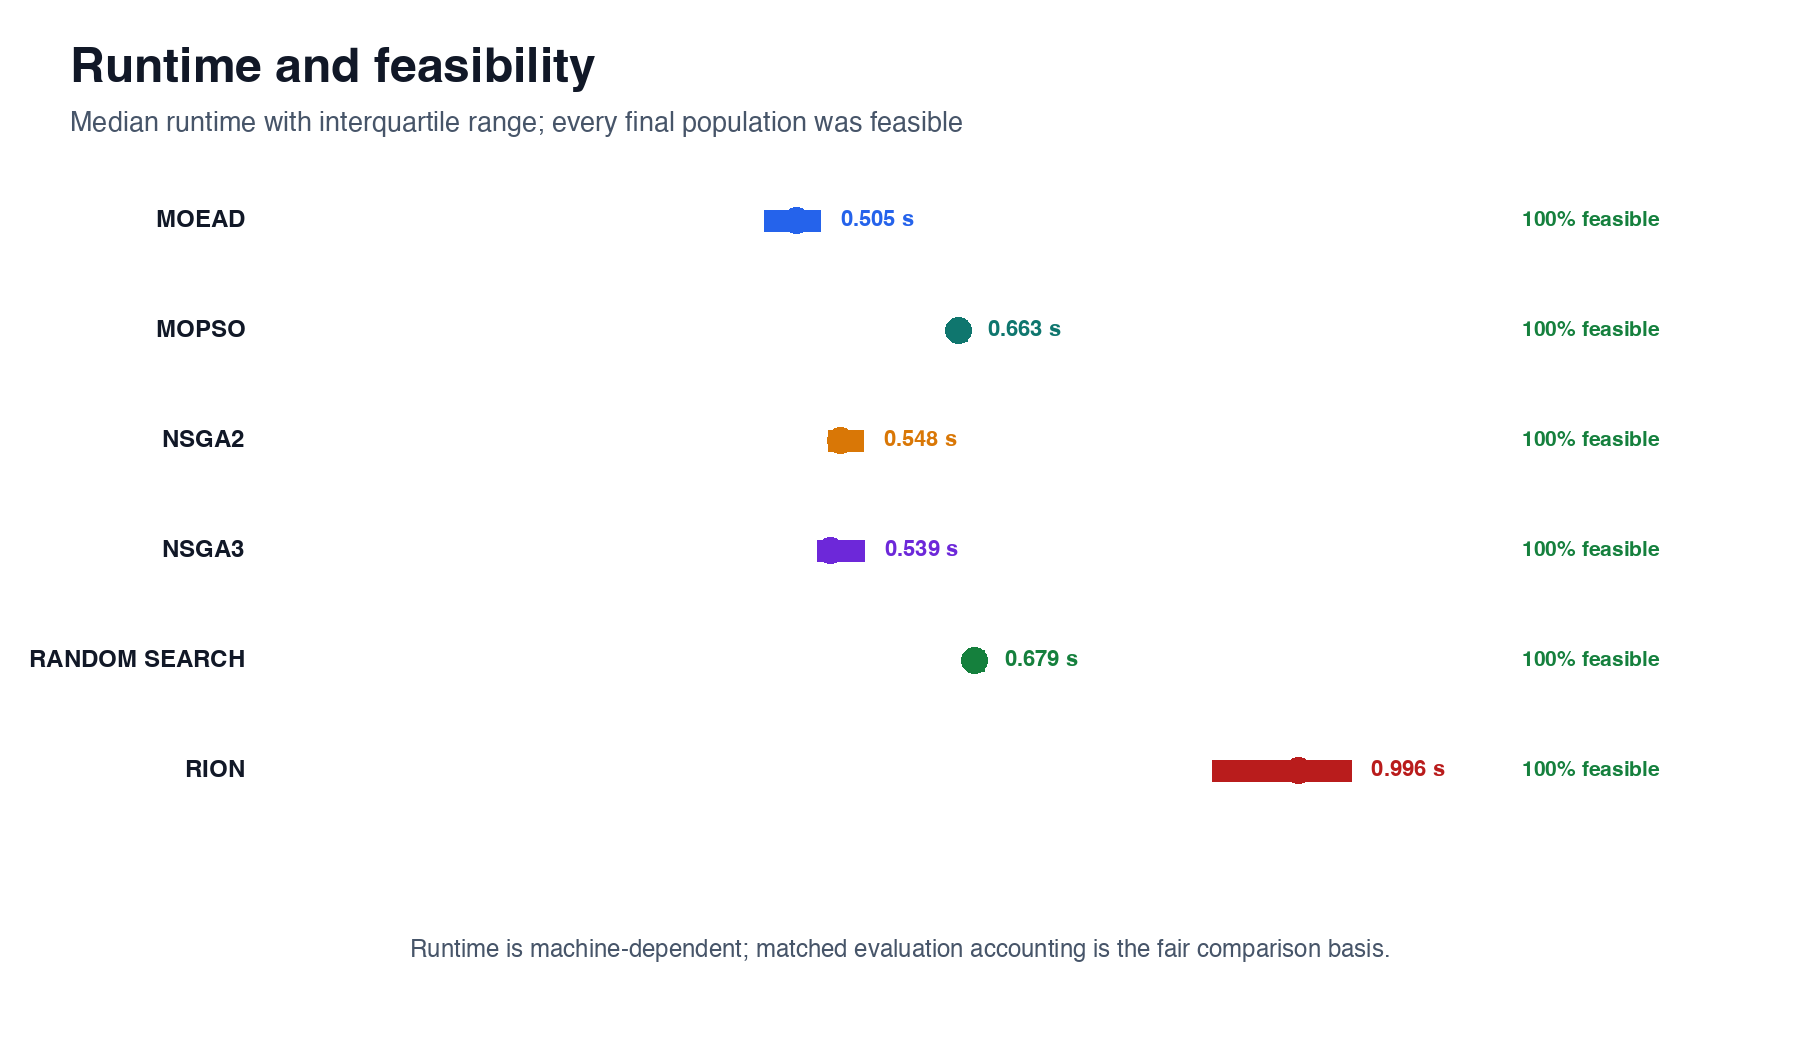
\includegraphics[width=\textwidth]{runtime_feasibility.png}\caption{Final benchmark runtime and feasibility. Runtime is descriptive and machine-dependent.}\end{figure}

Median runtimes were 0.505 s for MOEA/D, 0.548 s for NSGA-II, 0.539 s for NSGA-III, 0.663 s for MOPSO, 0.679 s for random search, and 0.996 s for RION. RION's additional cost reflects its inner-swarm work under the same evaluation-accounting contract.

\begin{figure}[H]\centering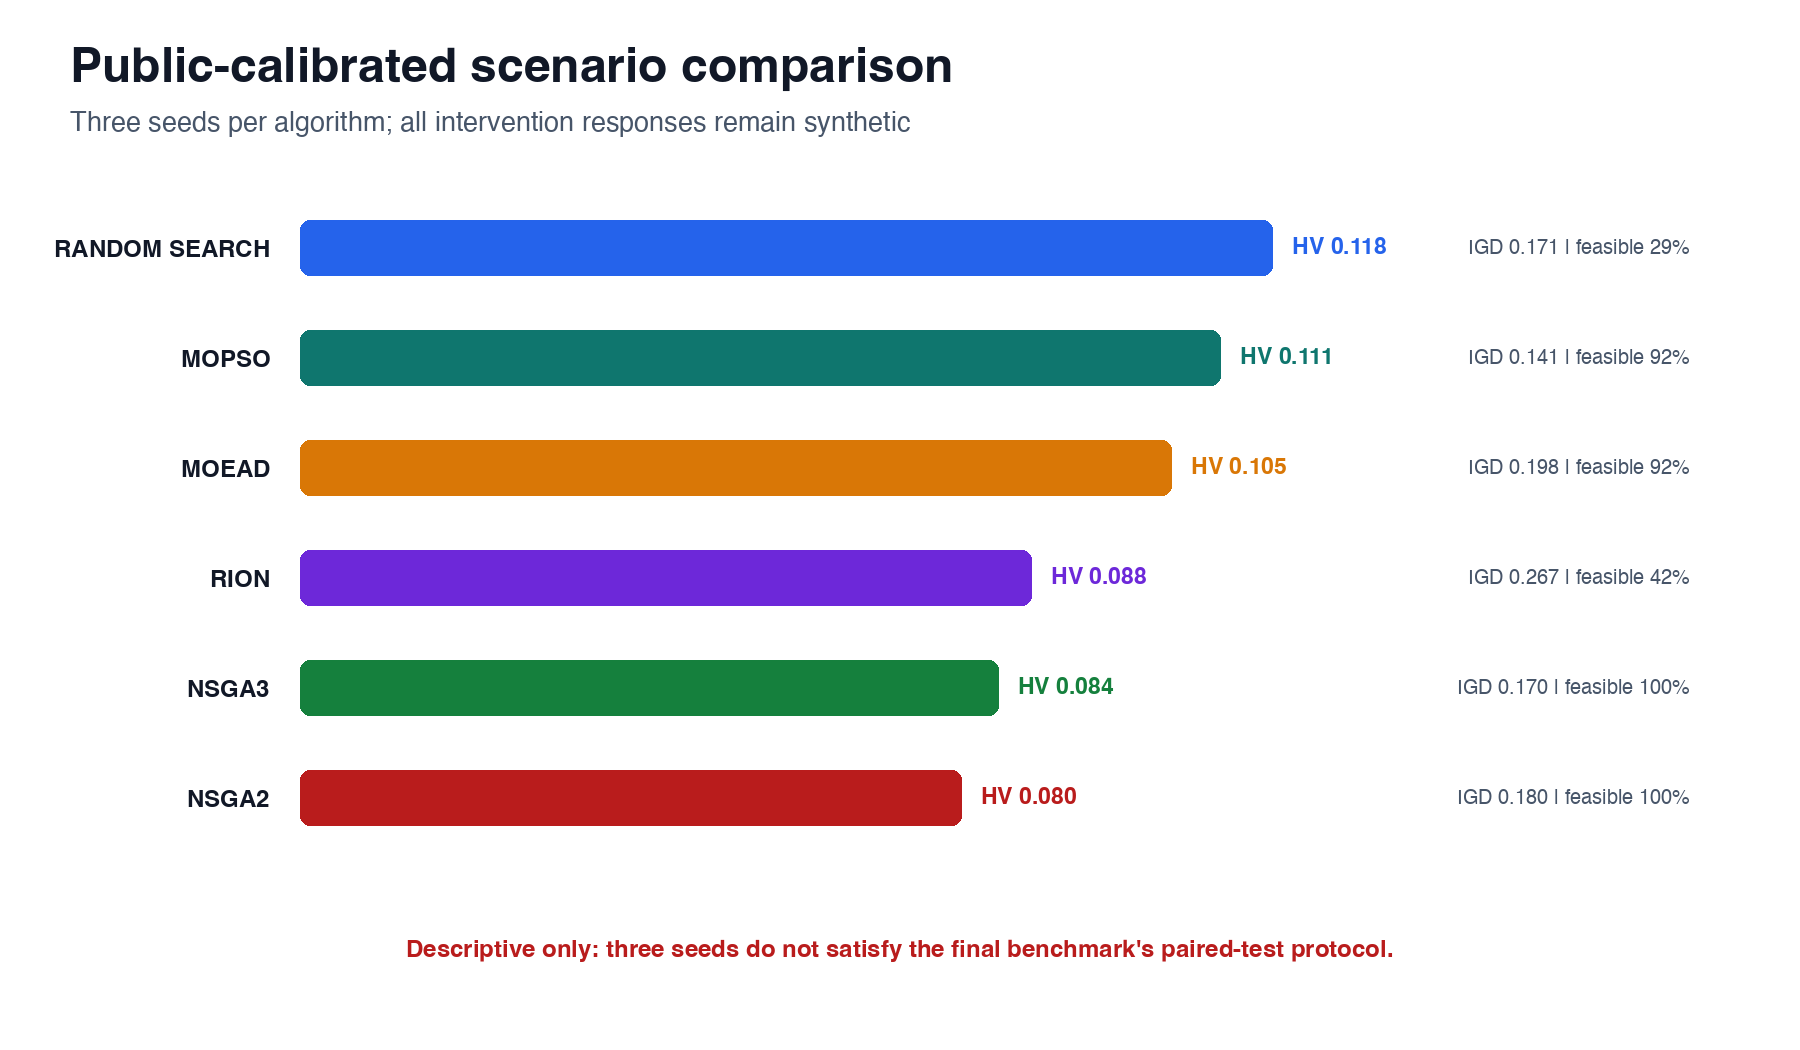
\includegraphics[width=\textwidth]{public_algorithm_comparison.png}\caption{Algorithm summaries for the 18-run public-calibrated scenario protocol.}\end{figure}

In the public-calibrated study, random search had the highest descriptive median hypervolume (0.117516), MOPSO 0.111222, and MOEA/D 0.105284. Feasible population rates varied from 0.2917 for random search to 1.0 for NSGA-II and NSGA-III. With only three seeds, the project does not run the final benchmark's inferential protocol or claim a winner.

\chapter{Departmental Resource Allocation Recommendations}
\begin{figure}[H]\centering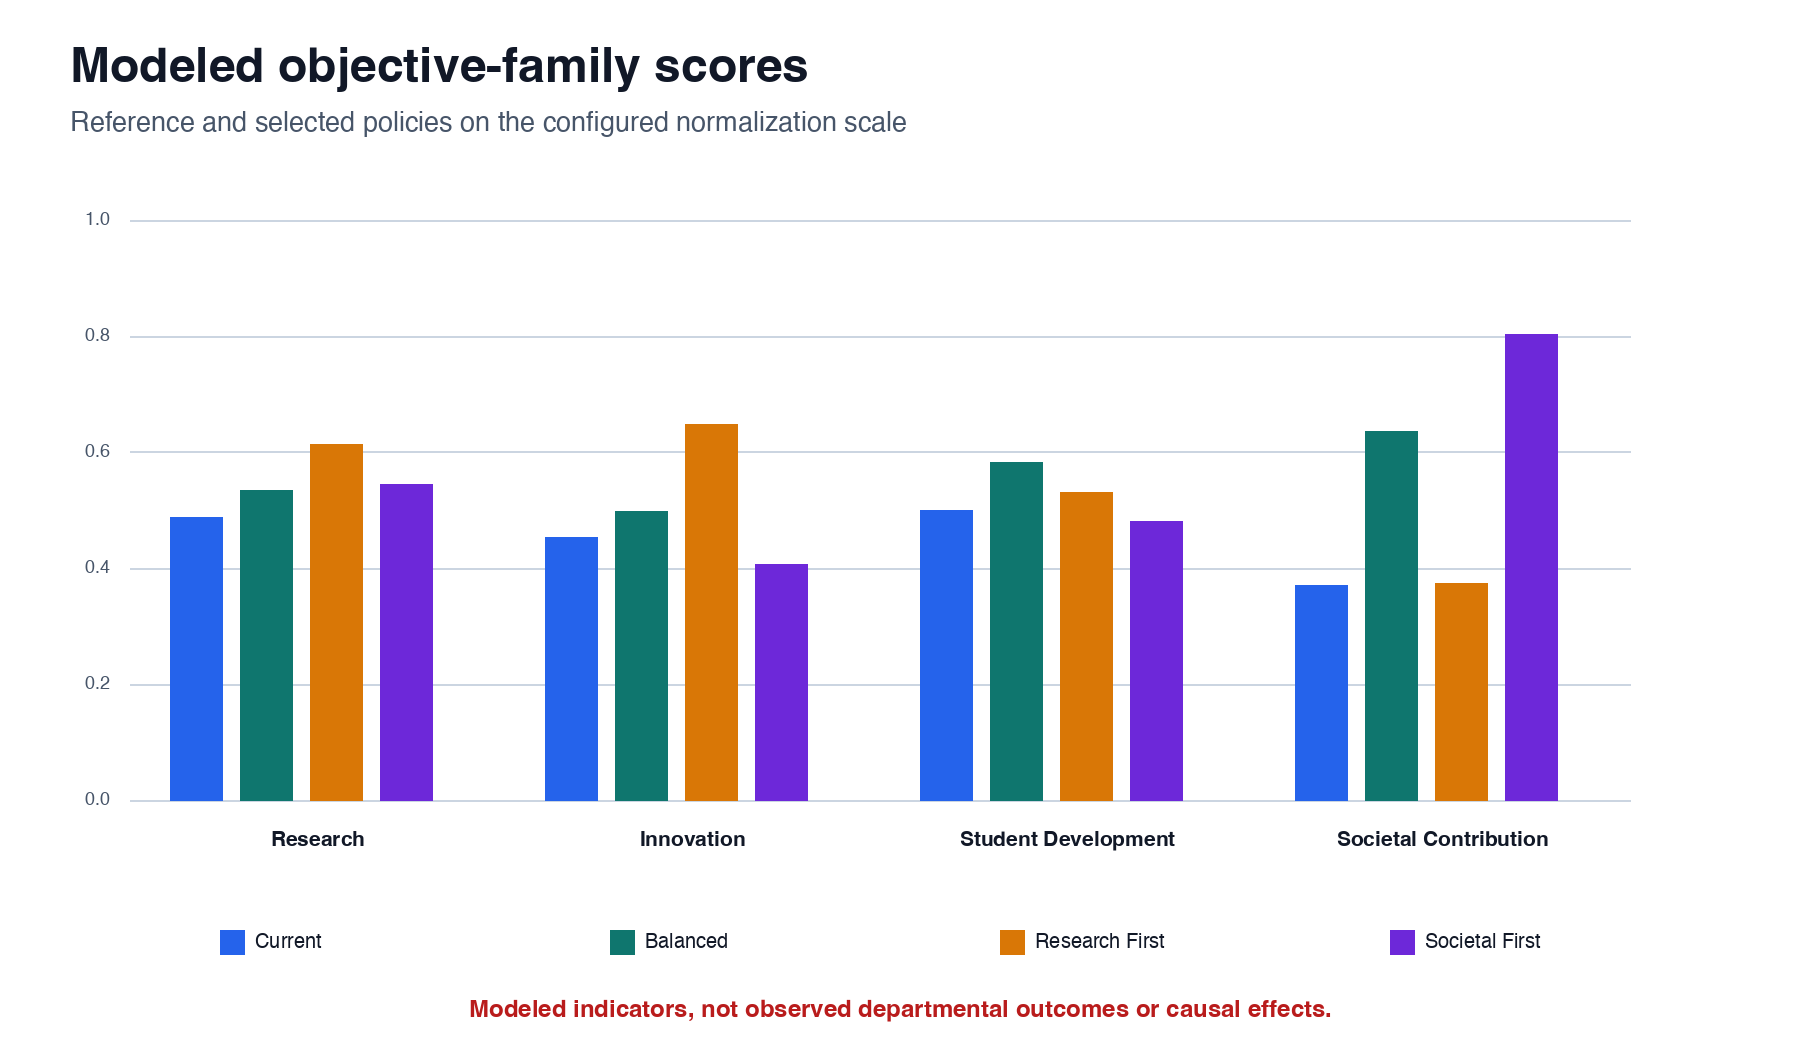
\includegraphics[width=\textwidth]{objective_scores.png}\caption{Modeled four-family objective benefits for the reference and selected public-calibrated strategies.}\end{figure}

The reference modeled benefits are 0.486839 (research), 0.451901 (innovation), 0.499402 (student development), and 0.369705 (societal contribution). The balanced selection uses INR 35.575 million, leaves INR 0.425 million headroom, and yields modeled benefits 0.533991, 0.497971, 0.581746, and 0.634732. The research and innovation profiles select the same MOEA/D candidate, while balanced and student profiles select the same MOPSO candidate; the UI discloses these duplicates.

\begin{figure}[H]\centering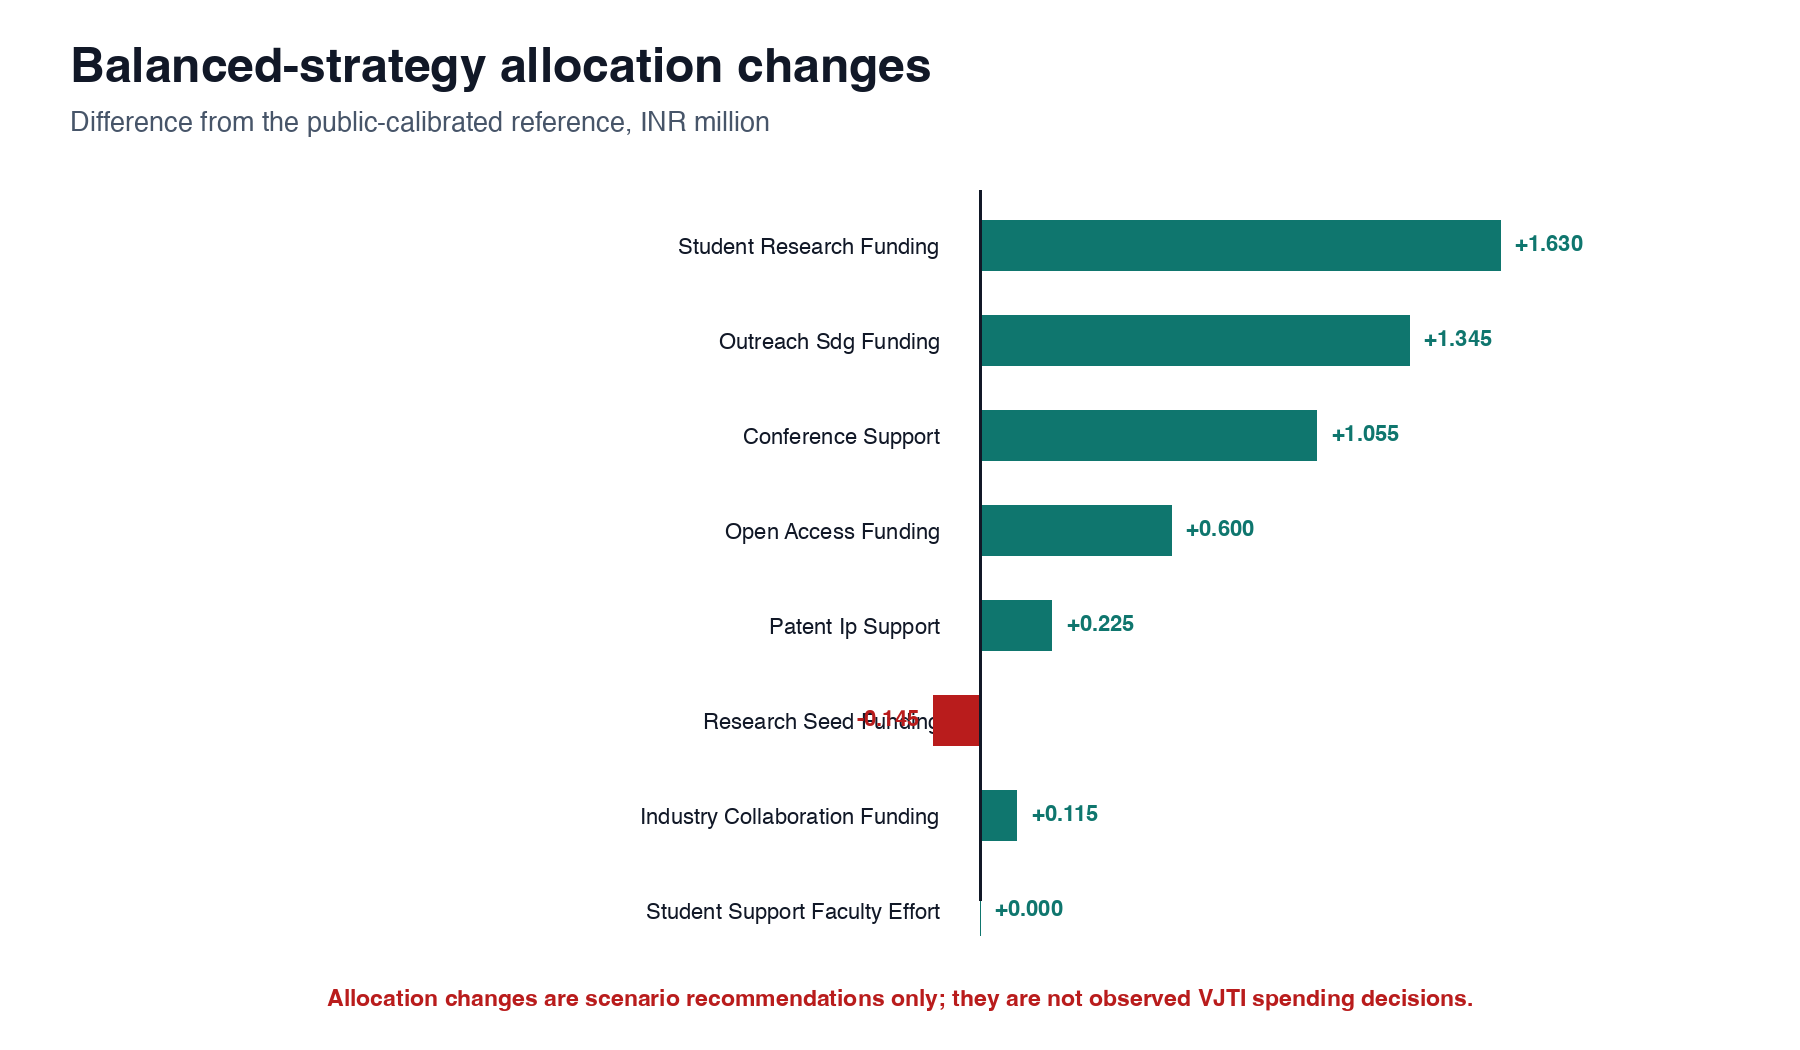
\includegraphics[width=\textwidth]{allocation_changes.png}\caption{Balanced-policy direct funding changes relative to the public-calibrated reference.}\end{figure}

The largest balanced-strategy modeled changes include +INR 1.630 million in student research funding, +INR 1.345 million in outreach/SDG funding, +INR 1.055 million in conference support, and +INR 0.600 million in open-access funding. Research seed funding decreases by INR 0.145 million. These are scenario actions inside an illustrative model, not observed budget decisions or guaranteed improvements.

\chapter{Robustness and Sensitivity Analysis}
\begin{figure}[H]\centering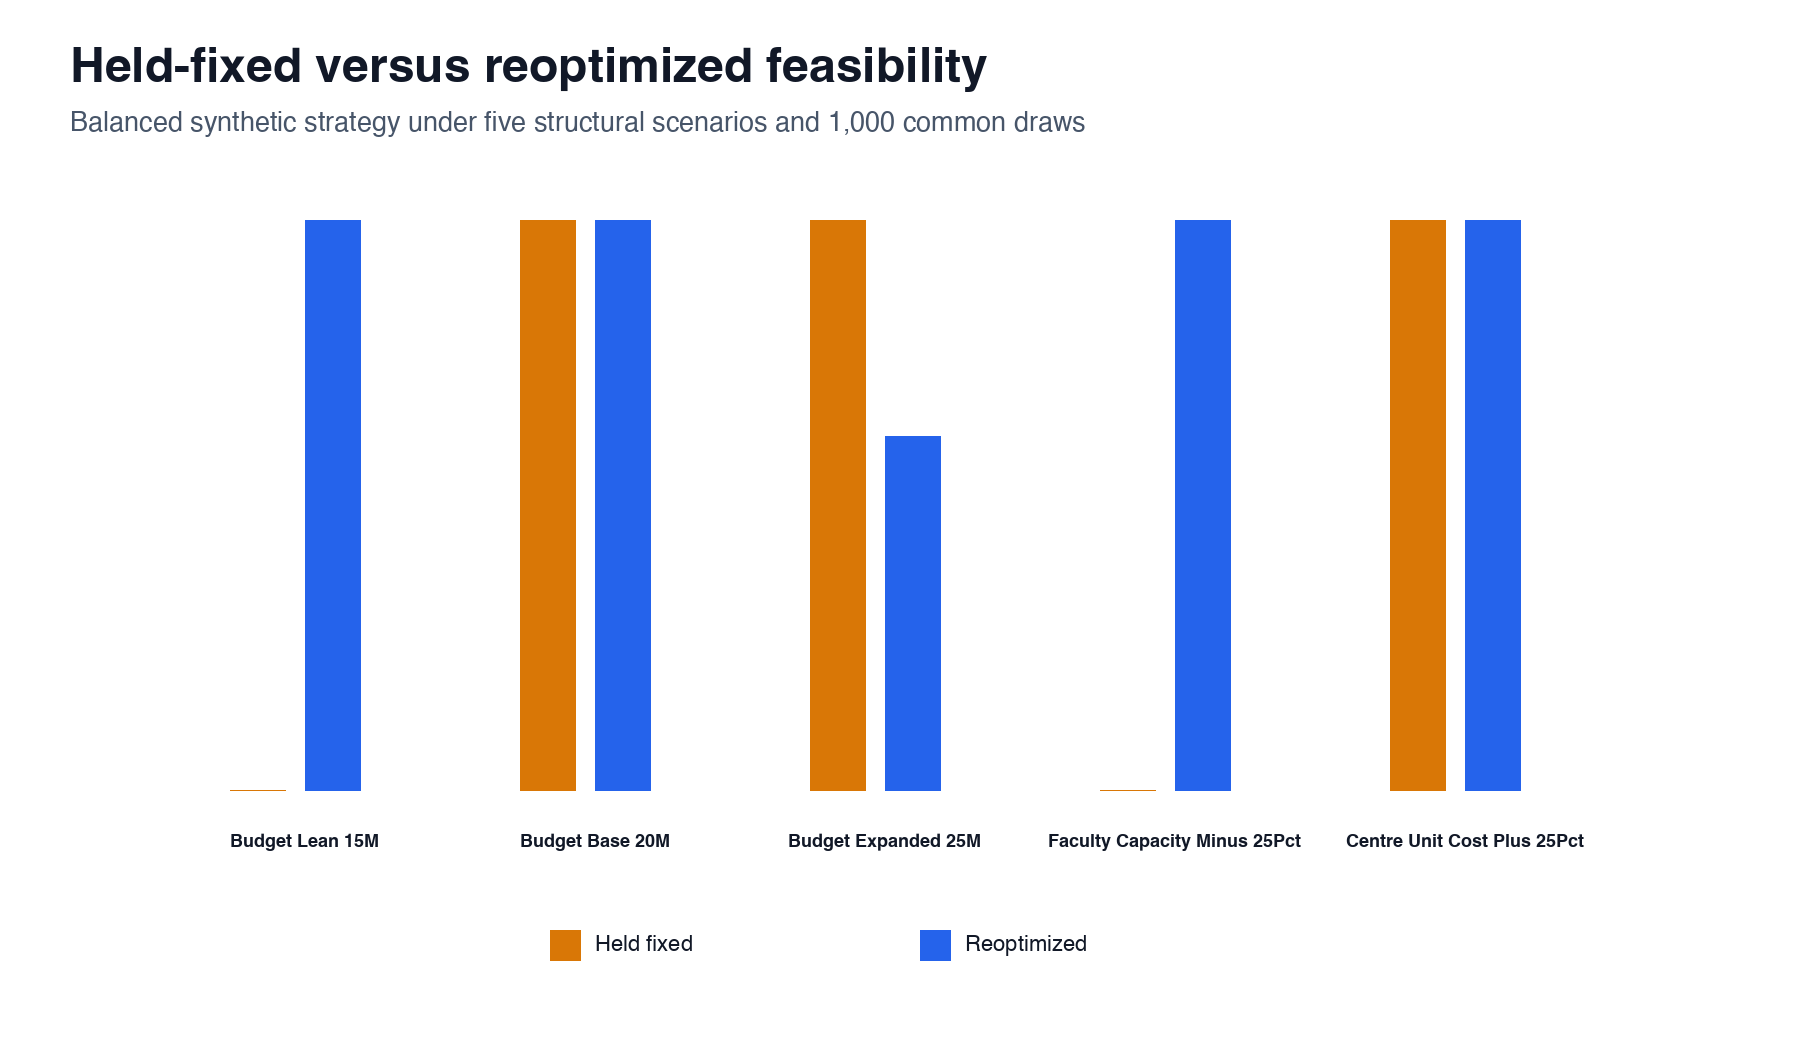
\includegraphics[width=\textwidth]{robustness.png}\caption{Held-fixed and reoptimized feasibility probabilities for the balanced synthetic strategy.}\end{figure}

Robustness explicitly separates evaluating a fixed baseline allocation under a changed scenario from rerunning the optimizer. Under the INR 15 million lean budget, the held-fixed INR 19.9 million strategy is infeasible with probability zero, whereas the reoptimized strategy is feasible in all 1,000 draws but has lower mean modeled papers (31.40 versus 41.15). Under the INR 25 million expanded budget, reoptimization increases modeled mean papers by 2.05 but its feasibility probability is 0.62 because uncertainty in cost is retained. A 25\% faculty-capacity reduction also makes the held-fixed strategy infeasible, while reoptimization restores feasibility.

Low, base, and high uncertainty assumptions are stored separately. Patent-cost and compute-cost shocks that are absent from the legacy decision vector are reported as unsupported rather than simulated with invented variables. The public-calibrated model does include corresponding decisions, but their response adjustments remain versioned local scenario assumptions.

\chapter{Testing and Verification}
\begin{figure}[H]\centering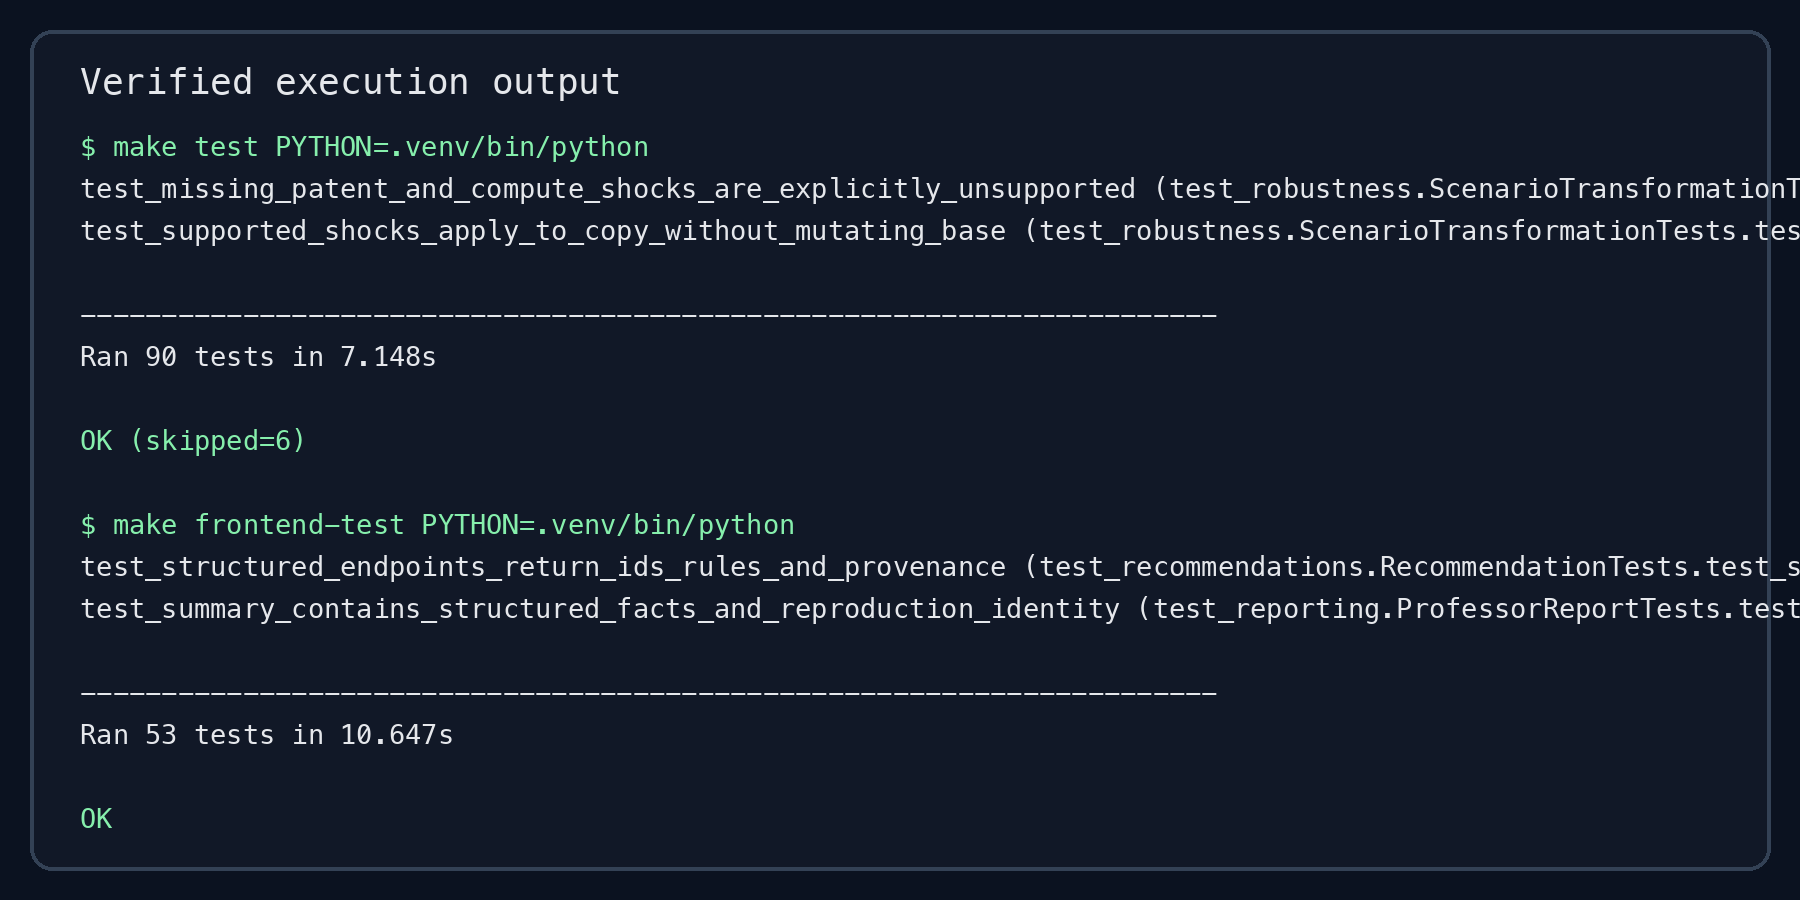
\includegraphics[width=\textwidth]{verification_output.png}\caption{Exact final lines rendered from the captured backend and Streamlit/API test logs.}\end{figure}

The backend command ran 90 tests in 7.148 seconds: 84 passed and six optional OpenMP-native PSO tests were skipped. The frontend command ran 53 tests in 10.647 seconds with no failures. Coverage includes schema failures, leakage, hand-solvable DEA frontiers, conformal quantiles, repair and constraints, algorithm contracts, matched budgets, resume behavior, metric fixtures, public evidence boundaries, recommendation reconciliation, explanation fallback, objective-score reconstruction, and live scenario execution through FastAPI.

Independent completion audits recompute final hypervolume by rectangle-union inclusion--exclusion and IGD by direct distance for every final run. The VJTI audit records 20 passed checks, zero failed checks, and three evidence gaps. Gaps are not converted into software failures or hidden successes.

\chapter{Limitations and Future Scope}
The principal limitation is evidence, not optimizer availability. The repository has no longitudinal observed CE\&IT department panel connecting allocations, carry-overs, faculty effort, and subsequent outcomes. It has no comparable complete public department cohort for DEA and no real intervention-response test set. Public institute totals cannot substitute for department observations. Therefore, predictive accuracy on the generator cannot establish causal allocation effects.

The legacy final benchmark has only one varying supported objective, so three algorithm families designed for many-objective diversity are tested structurally but not in a real four-objective department study. The public-calibrated study represents all four families but uses only three seeds and fully synthetic responses. Target-cost search is heuristic and returns a feasible upper bound, not a proof of a global minimum. Runtime is local and the live service uses a single persisted worker.

Stronger validation requires aligned multi-year department records for budgets, activity allocations, faculty effort, research assistance, compute use, and KPI outcomes; comparable departments with common definitions and base years; preregistered temporal splits; and, for causal claims, an appropriate quasi-experimental or randomized allocation design. Network DEA and multi-period optimization should remain deferred until observed stage-link and carry-over variables exist.

\chapter{Conclusion}
Beyond Ranking has progressed from a hybrid-algorithm proposal into a complete evidence-aware optimization prototype. It includes a validated data layer, provenance, DEA, KPI models, a mixed-variable evaluator, six algorithms, matched-budget benchmarks, statistical comparisons, robustness, strategy and target-cost reports, independent audits, and a live Streamlit/FastAPI interface. The final benchmark demonstrates reproducible method differences, with MOPSO and MOEA/D leading the frozen synthetic fixture, while the dashboard converts saved and live results into traceable departmental actions.

The scientifically important outcome is the boundary around those capabilities. The system can show feasible modeled trade-offs and explain why a strategy was selected. It cannot yet claim that a proposed allocation will improve actual VJTI outcomes. By making that boundary visible in artifacts, tests, reports, and UI, the project satisfies the requirement for live, understandable optimization without overstating the evidence.

\bibliographystyle{ieeetr}
\bibliography{references}

\appendix
\chapter{Reproduction Commands}
\begin{verbatim}
python3 -m venv .venv
source .venv/bin/activate
python -m pip install -r requirements.txt
python -m pip install -r requirements-ui.txt

make test PYTHON=.venv/bin/python
make frontend-test PYTHON=.venv/bin/python
make public-data
make evidence-models
make public-allocation
make public-experiments
make public-completion-audit

# terminal 1
make frontend-api PYTHON=.venv/bin/python
# terminal 2
make frontend-dev PYTHON=.venv/bin/python

.venv/bin/python report/generate_report_assets.py
/Applications/ChatGPT.app/Contents/Resources/tectonic/tectonic \
  Beyond_Ranking_Final_Report.tex
\end{verbatim}

\chapter{Artifact Evidence Map}
\small
\begin{longtable}{p{0.30\textwidth}p{0.62\textwidth}}
\toprule Artifact & Report use\\\midrule
\artifact{results/benchmarks/phase6-final-synthetic-25seeds-v1/per_seed_metrics.csv} & 150 final run observations\\
\artifact{results/benchmarks/phase6-final-synthetic-25seeds-v1/summary_median_iqr.csv} & Benchmark medians and IQRs\\
\artifact{results/benchmarks/phase6-final-synthetic-25seeds-v1/statistical_tests.csv} & Wilcoxon, rank-biserial, Holm results\\
\artifact{artifacts/public_experiments/vjti_v1/algorithm_summary.csv} & 18-run public-calibrated comparison\\
\artifact{artifacts/public_experiments/vjti_v1/strategy_allocations.csv} & Allocation recommendations and units\\
\artifact{artifacts/public_experiments/vjti_v1/strategy_objectives.csv} & Four modeled objective benefits\\
\artifact{artifacts/evidence_modeling/vjti_v1/model_metrics.csv} & Nine-KPI generator-validation metrics\\
\artifact{results/robustness/phase6b-synthetic-v1/fixed_vs_reoptimized_comparison.csv} & Robustness modes and deltas\\
\artifact{artifacts/public_data/vjti_ceit_v1/source_register.csv} & Seven retained official source snapshots\\
\artifact{artifacts/public_audit/vjti_v1/audit_checks.csv} & Public completion audit\\\bottomrule
\end{longtable}

\chapter{Metric Definitions and Claim Checklist}
Hypervolume is the dominated volume bounded by the frozen reference point. IGD is the mean distance from each point on the pooled reference front to its nearest archive point. Spacing measures nearest-neighbor distance variability. Feasibility rate is the proportion of final population candidates satisfying all named constraints. Runtime is wall-clock implementation time and is not hardware-independent.

Before using any recommendation, verify: evidence lane; scenario and model hashes; units and base year; candidate feasibility; out-of-support flags; KPI intervals; duplicate strategy status; selection rule; held-fixed versus reoptimized mode; and whether the claim is descriptive, modeled, predictive, or causal. The current report contains no causal departmental claim.

\end{document}
